\documentclass[a4paper]{article}

\usepackage{pgfplots}

\pgfplotsset{
	compat=1.8,
	xlabel=$x$,
	ylabel=$y$,
	zlabel=$z$,
	domain=-4e4:4e4,
	ticklabel style={draw=red},
}

\begin{document}

	%\tracingcommands=2\tracingmacros=2
\parskip=1cm

\fbox{%
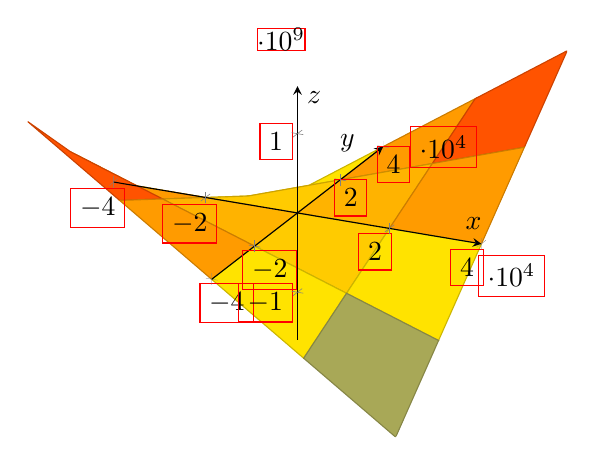
\begin{tikzpicture}
    \begin{axis}[
        axis lines=center,
        axis on top,
        samples=5,
        xtick=data, ytick=data,
    ]
        \addplot3[surf] {x*y};
    \end{axis}
\end{tikzpicture}}%

\fbox{%
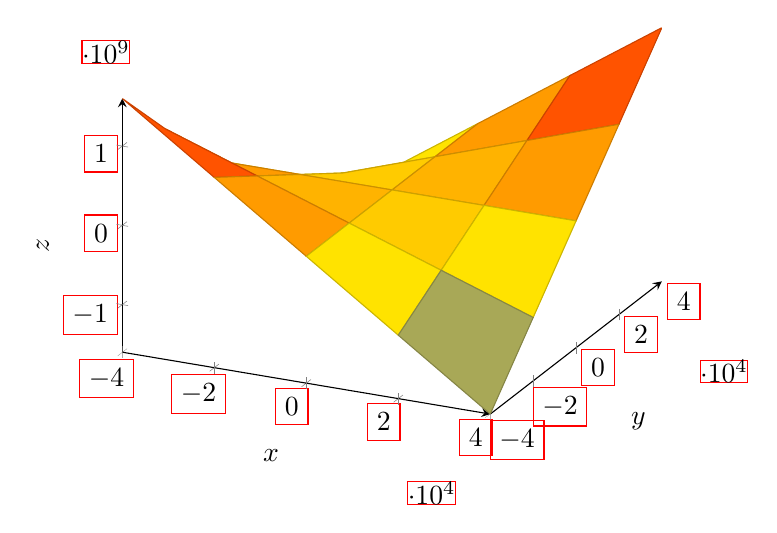
\begin{tikzpicture}
    \begin{axis}[
        axis lines=left,
        samples=5,
        xtick=data, ytick=data,
    ]
        \addplot3[surf] {x*y};
    \end{axis}
\end{tikzpicture}%
}%

\fbox{%
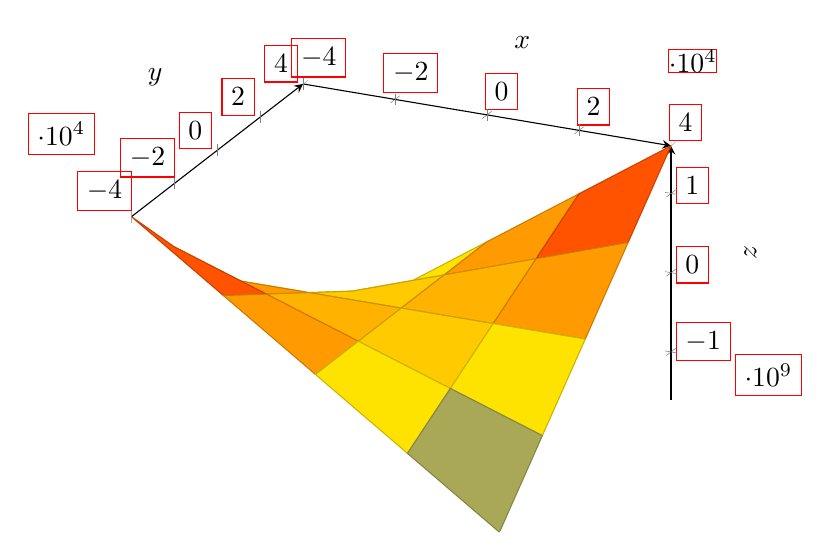
\begin{tikzpicture}
    \begin{axis}[
        axis lines=right,
        samples=5,
        xtick=data, ytick=data,
    ]
        \addplot3[surf] {x*y};
    \end{axis}
\end{tikzpicture}%
}

\end{document}
